\chapter{Maximum independent set formulation of the partial row/column assignment problem} \label{chap:independent_set}

With the framework introduced in Section \ref{sec:hot_restart}, we basically translated the problem of the assignment of nonzeros to $A_r$ and $A_c$ (which is already another formulation of the matrix partitioning problem with the medium grain model) to the problem of an efficient computation of a permutation of the indices $0,\dots,m+n-1$. In this chapter, we will propose a method for this vector computation problem, which relies on concepts of the field of graph theory.

The main idea is somewhat similar to the principle that lead us to the development of the Separated Block Diagonal form of order 2 in Section \ref{sec:sbd2}. In that particular form of a partitioned matrix, as already argued, the blocks $\ddot{A}_{00}$ and $\ddot{A}_{44}$ are interesting, because they contain ``independent'' nonzeros. More specifically, those rows and columnsare fully assigned to a processor and whose nonzeros do not have any neighbor (a nonzero in the same row or column) which had a cut column/row. These nonzeros, then, can be assigned anywhere and do not cause communication.

The term \emph{independent}, in this reasoning, has to be defined very carefully: we want to look for a subset of the indices $\{0,\dots,m+n-1\}$ which does not cause any communication, whenever we fully assign its rows to $A_r$ and its columns to $A_c$. With this definition, our goal is clear: we want to assign as much nonzeros as possible in this way, obtaining a low upper bound on the communication volume, which can be computed during the creation of $A_r$ and $A_c$.

To do so, we can employ a very well studied object in graph theory: the \textbf{maximum independent set}. However, this requires a correct translation of our sparse matrix into a graph, described in Section \ref{sec:is_graph}. In Section \ref{sec:is_comp}, instead, we delve a little more into the graph theory required and describe the actual algorithm used to compute the maximum independent set in such graph.

\section{Graph construction} \label{sec:is_graph}

We need to construct the graph correctly from our sparse matrix, in order to retrieve our desired information. In our case, we can simply consider the graph whose adjacency matrix is none other than the sparsity pattern of our matrix $A$. This exact same formulation has already been studied, for the matrix partitioning problem, under the name of \emph{bipartite graph model} by Hendrickson and Kolda \cite{hendrickson}; in the same work, the authors, after constructing the graph, discuss different algorithms for bipartite graph partitioning and come to the conclusion that the best strategy is using multilevel methods with Fiduccia-Mattheyses refinement.

More explicitly, in this graph formulation, we have that rows and columns are vertices, and we have an edge $(i,j)$ if $a_{ij} \neq 0$. It is fairly clear that the resulting graph is bipartite, because an edge connects only rows with columns.

An example of such translation from matrix to graph is shown in Figure \ref{fig:bipartite_graph}, where we start from the matrix given in Figure \ref{fig:partition}. 

\begin{figure}[h]
	\centering
	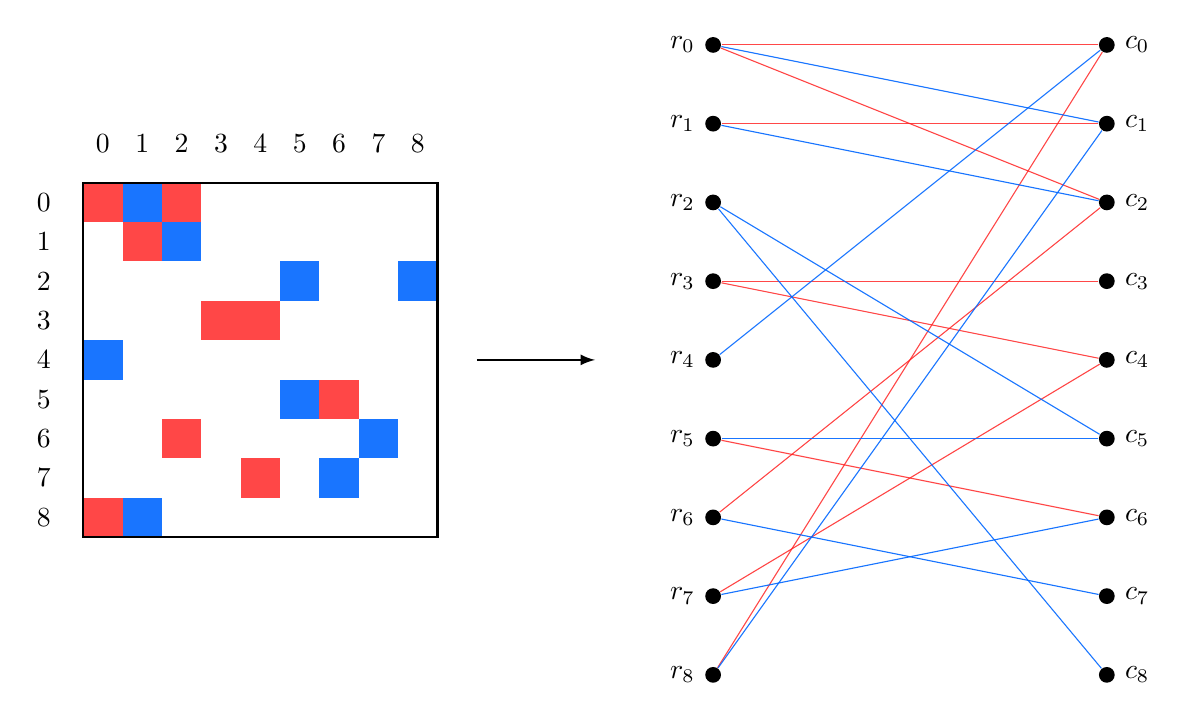
\begin{tikzpicture}[scale=0.5]
		\tikzstyle{myred}=[red!90,opacity=.8]
		\tikzstyle{myblue}=[blue!60!cyan,opacity=.9]
		\tikzstyle{mypurple}=[purple!80!blue,opacity=.9]
		\tikzstyle{myarrow}=[line width=1.3pt,>=latex,->]
		\tikzstyle{vertex} = [fill,shape=circle,node distance=100pt,minimum size=0.2cm,inner sep = 0pt]
		\foreach \x / \y in {1/1,1/3,2/2,4/5,4/4,7/3,8/5,6/7,9/1} { \fill[myred] ({\y-1},{-\x+1}) rectangle +(1,-1);}
		\foreach \x / \y in {1/2,2/3,3/6,3/9,6/6,5/1,7/8,8/7,9/2} { \fill[myblue] ({\y-1},{-\x+1}) rectangle +(1,-1);}
%		\draw[semithick] (0,-9) grid (9,0);
		\draw[thick] (0,-9) rectangle (9,0);

		\draw[myarrow,thick] (10,-4.5) -- (13,-4.5);

		\foreach \x in {0,...,8} { 
			\node[vertex,label=left:\(r_{\x}\)] (r\x) at (16,{3.5-2*\x}) {}; 
			\node[vertex,label=right:\(c_{\x}\)] (c\x) at (26,{3.5-2*\x}) {};
			\node at (-1,{-\x-0.5}) {\x};
			\node at (\x+0.5,1) {\x};
		}

		\foreach \x / \y in {0/0,0/2,1/1,3/4,3/3,6/2,7/4,5/6,8/0} { \draw[myred] (r\x) -- (c\y);}
		\foreach \x / \y in {0/1,1/2,2/5,2/8,5/5,4/0,6/7,7/6,8/1} { \draw[myblue] (r\x) -- (c\y);} 
	\end{tikzpicture}
	\caption{Graph constructed using the sparsity pattern of the matrix of Figure \ref{fig:partition} as adjacency matrix (rows and columns are vertices, nonzeros are edges). The edge color is the same of the corresponding nonzero, but only to facilitate the understanding of this translation; in reality there is no distinction between edges. In the bipartite graph, with $r_i$ we denote row $i$, whereas with $c_j$ we denote column $j$.} \label{fig:bipartite_graph}
\end{figure}

\section{The maximum independent set and its computation} \label{sec:is_comp}

In this section, we will give an extensive overview of the maximum independent set problem, discuss its complexity and the relation with other famous problems in graph theory, and, lastly, give an efficient algorithm that can be used in our case, with a bipartite graph.

\subsection{Maximum independent set}

The concept of independent set is closely related to the concept of \emph{vertex cover} \cite{np_book}: let $G=(V,E)$ be an undirected graph.

\begin{definition}[Independent set]
	An \emph{independent set} is a subset $V' \subseteq V$ such that $ \forall u,v \in V'$, $(u,v) \notin E$.
	The \emph{maximum} independent set is the independent set of $G$ with maximum cardinality.
\end{definition}

\begin{definition}[Vertex cover]
	A \emph{vertex cover} is a subset $V' \subseteq V$ such that $\forall (u,v) \in E$ we have $u \in V' \vee v \in V'$, i.e. at least one of the endpoint of any edge is in the cover. The \emph{minimum} vertex cover is the vertex cover of $G$ with minimum cardinality.
\end{definition}

A graphical depiction of two independent sets is shown in Figure \ref{fig:is_example}.

\begin{figure}[h]
	\centering
	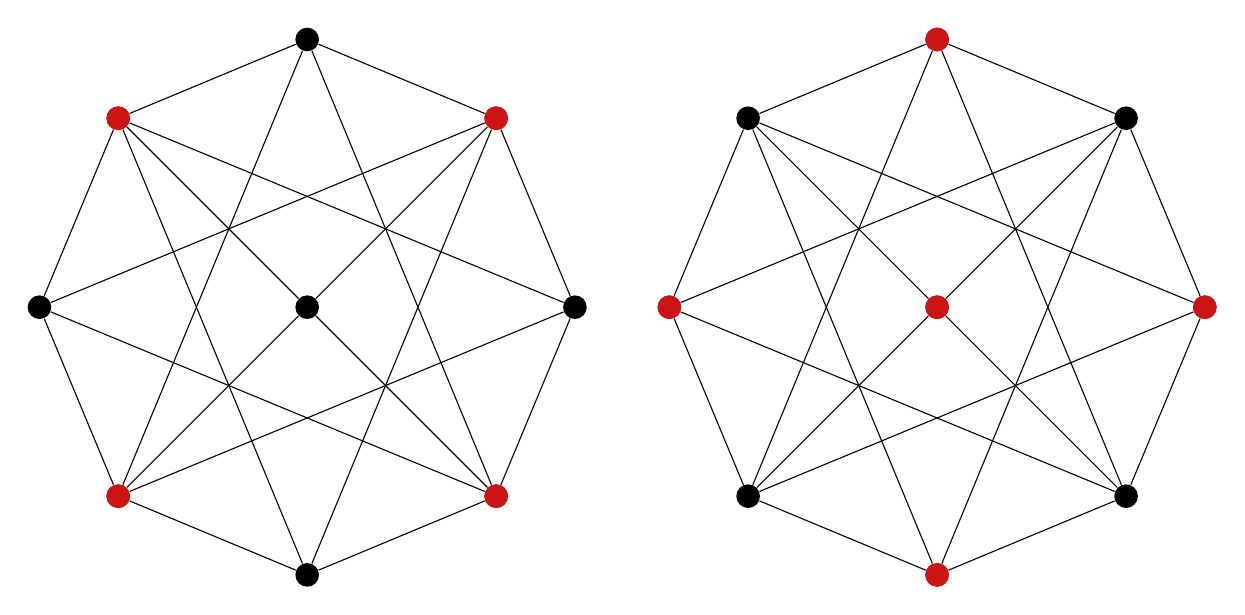
\begin{tikzpicture}[scale=0.2]
		\tikzstyle{myred}=[red!90,opacity=.8]
		\tikzstyle{myblue}=[blue!60!cyan,opacity=.9]
		\tikzstyle{mypurple}=[purple!80!blue,opacity=.9]
		\tikzstyle{myarrow}=[line width=1.3pt,>=latex,->]
		\tikzstyle{vertex} = [fill,shape=circle,node distance=100pt,minimum size=0.3cm,inner sep = 0pt]

		\foreach \x / \y / \z in {17/0/1,12/12/2,-17/0/5,-12/12/4,12/-12/8,0/17/3,0/-17/7,-12/-12/6,0/0/0} { \node[vertex] (n\z) at (\x,\y) {};}
		\foreach \x in {2,4,...,8} { \draw (n\x) -- (n0);}

		\draw (n1) -- (n2) -- (n3) -- (n4) -- (n5) -- (n6) -- (n7) -- (n8) -- (n1);
		\draw (n8) -- (n3) -- (n6);
		\draw (n2) -- (n7) -- (n4);
		\draw (n2) -- (n5) -- (n8);
		\draw (n4) -- (n1) -- (n6);


		\foreach \x in {2,4,6,8} {\node[vertex,myred] at (n\x) {}; }

		\foreach \x / \y / \z in {17/0/1,12/12/2,-17/0/5,-12/12/4,12/-12/8,0/17/3,0/-17/7,-12/-12/6,0/0/0} { \node[vertex] (m\z) at (40+\x,\y) {};}
		\foreach \x in {2,4,...,8} { \draw (m\x) -- (m0);}

		\draw (m1) -- (m2) -- (m3) -- (m4) -- (m5) -- (m6) -- (m7) -- (m8) -- (m1);
		\draw (m8) -- (m3) -- (m6);
		\draw (m2) -- (m7) -- (m4);
		\draw (m2) -- (m5) -- (m8);
		\draw (m4) -- (m1) -- (m6);
		\foreach \x in {0,1,3,5,7} {\node[vertex,myred] at (m\x) {}; }

	\end{tikzpicture}
	\caption{Two different independent sets (red vertices) on an example graph. The two independent sets have different cardinality, and the one on the right is the maximum independent set.} \label{fig:is_example}
\end{figure}

\begin{lemma} 
	\label{lemma:is}
	Given a graph $G$, $V'$ is a vertex cover set if and only if $V \setminus V'$ is a independent set.
\end{lemma}
\begin{proof}
	Let $V'$ be a vertex cover, i.e. $\forall (u,v) \in E$, we have that $u \in V'$ or $v \in V'$. This is equivalent to say that $\forall u,v \in V \setminus V'$ we have that $(u,v) \notin E$, which is the definition of independent set.
\end{proof}
As the decision variant of the problem of finding a vertex cover is NP-complete \cite[Theorem 3.3]{np_book}, it follows from this lemma that also finding an independent set in a graph is NP-Complete; the main consequence of this result is that we cannot solve this problem directly for a generic graph, as it would be as hard as our original matrix partitioning problem. Luckily, we are dealing with a particular kind of graph, which simplifies greatly the complexity of the computation of the maximum independent set.

Before exploiting the bipartiteness of our graph, we need to make an additional observation: Lemma \ref{lemma:is} states that the vertex cover problem and independent set cover are complementary. Therefore, computing the maximum independent set is equivalent to computing the minimum vertex cover.

This is particularly useful in our case, because we can use the fact that our graph is bipartite and employ K\H{o}nig's Theorem \cite{konig}, which states that, in any bipartite graph, the size of the maximum matching is the size of the minimum vertex cover. 

Because of this relationship, it is convenient to recall the definition of (maximum) matching.

\begin{definition}[Matching]
	Let $G=(V,E)$ be a graph. A \emph{matching} $M \subseteq E$ is a set of edges such that at most one edge is incident to each vertex $v \in V$. We say that a vertex $v \in V$ is matched by $M$ if an edge in $M$ is incident to $v$. The \emph{maximum} matching is a matching of maximum cardinality.
\end{definition}

In Figure \ref{fig:is_example} we can indeed observe that every edge is incident to a black vertex.

Because of K\H{o}nig's Theorem, then, it suffices to find an efficient algorithm for the computation of the maximum matching on a bipartite graph, then finding the minimum vertex cover and finally, by taking the complementary set, obtaining the maximum independent set.

\subsection{The Hopcroft-Karp algorithm for bipartite matching}

An efficient algorithm for the computation of the maximum matching of a bipartite graph is the Hopcroft-Karp algorithm \cite{hopcroft_karp}, devised in 1973. The running time of this algorithm is $\mathcal{O}\left( |E|\sqrt{|V|} \right)$, a considerable improvement over the famous Ford-Fulkerson algorithm which, for bipartite graphs, has a running time of $\mathcal{O}\left( |V||E| \right)$. Note that we can do a comparison with the Ford-Fulkerson algorithm, which is technically meant for the maximum flow problem, because we can modify a bipartite graph such that the maximum flow in the modified graph corresponds to a maximum matching in the original graph. 

Both these two algorithms rely on the concept of \emph{augmenting paths}, even though, as they are meant for solving different problems, the definitions are not exactly identical; in case of matching we have:

\begin{definition}[Augmenting path]
	Let $M$ be a matching on the graph $G=(V,E)$. The simple path $P$ is said to be \emph{augmenting} if it starts and ends on unmatched vertices, and its edges alternate between $E \setminus M$ and $M$ (i.e. alternating between the edges in the matching and the other edges).
\end{definition}

It is easy to see that if we have a matching $M$ and an augmenting path $P$, $M \oplus P$ is a matching of size $|M|+1$, where $M \oplus P := (M \setminus P) \cup (P \setminus M)$ denotes the \emph{symmetric difference} between $M$ and $P$. 

The general idea of the Hopcroft-Karp algorithm is to use these augmenting paths to progressively increase the size of the matching, as outlined in Algorithm \ref{alg:hopcroft-karp} \cite{hopcroft_karp}:

\begin{algorithm}[h]
	\begin{algorithmic}
	\Require{Bipartite graph $G=(V,E)$}
	\Ensure{Maximum matching $M$}
	\State $M \gets \varnothing$
	\Repeat
	\State $l_M \gets$ length of the shortest augmenting path, using the matching $M$
	\State $P \gets \{ P_1,\dots,P_k \}$, the maximal set of vertex-disjoint shortest augmenting paths of length $l_M$
	\State $M \gets M \oplus (P_1 \cup \dots \cup P_k )$
	\Until{ $P=\varnothing$}
\end{algorithmic}
\caption{Basic outline of the Hopcroft-Karp algorithm} \label{alg:hopcroft-karp}
\end{algorithm}

The core of this algorithm relies on finding all the shortest augmenting paths, and this is where the bipartiteness of the graph is fundamental (note that Algorithm \ref{alg:hopcroft-karp} is technically suitable for any graph). Let $L,R$ be the two disjoint sets of vertices such that $V = L \cup R$.

The procedure of computing $l_M$ and $P$, which is divided in three phases:

\begin{enumerate}
	\item \textbf{partitioning of the graph into layers}: the first layer $\Lambda_0$ is constructed with only the unmatched vertices in $L$, then in $\Lambda_1$ we place the vertices in $R$ connected to the nodes in $\Lambda_0$ (which, by definition of unmatched vertices of $L$, are not in $M$); this process is iterated such that $\Lambda_i$ contains vertices in $L$ if $i$ is even, and vertices of $R$ if $i$ is odd, and the traversed edges between the layers have to alternate between unmatched (from even layer to odd, i.e. from $L$ to $R$) and matched (between odd layer to even, i.e. from $R$ to $L$). This partitioning is performed with a \textbf{breadth-first search} and it terminates at layer $l_M$, where one (or more) free vertices in $R$ are reached.
	\item \textbf{collection of free vertices}: all the free vertices of $R$ discovered at layer $l_M$ (thus only the endpoints of a shortest augmenting path) are collected in a set $F$.
	\item \textbf{computation of the maximal set of vertex-disjoint shortest augmenting paths}: $P$ is computed using a \textbf{depth-first search} from $F$ to $L$, using the layers $\Lambda_i$, $i=1,\dots,k$ for the search. In particular, at each level we are only allowed to follow edges that lead to an unused vertex in the previous layer, and paths must alternate between matched and unmatched edges. Whenever we find an augmenting path we add it to $P$ and resume with the next vertex in $F$.
\end{enumerate}

Note that, by finding the maximal set of shortest augmenting paths, we need only $\mathcal{O}\left( \sqrt{|V|} \right)$ inner iterations inside Algorithm \ref{alg:hopcroft-karp}. This, combined with the fact that the breadth-first search and depth-first search have a running time of $\mathcal{O}(|E|)$, yields a total running time of $\mathcal{O} \left( |E|\sqrt{|V|} \right)$.
Furthermore, if we use the Hopcroft-Karp algorithm in our sparse graph constructed as in Section \ref{sec:is_graph}, the running time can be even considerably better (if there are not rows and columns particularly dense, in our graph we have that each vertex has just a handful of edges, resulting in fast search phases).

\section{Computation of the priority vector $v$ with the maximum independent set}

After having translated our matrix into a graph as in Section \ref{sec:is_graph} and having computed the maximum independent set as described in Section \ref{sec:is_comp}, we still have to compute our priority vector $v$, to be used in the same framework of Section \ref{sec:hot_restart}.

Similarly as done for all the methods described in Chapter \ref{chap:methods}, we will specify two ways of computing the vector $v$, one partition-oblivious and one partition-aware.

For the partition-oblivious version of the method, we can simply compute the maximum independent set on the graph constructed from the full matrix $A$, and then simply put first the indices corresponding to the independent set and then the others.

For the partition-aware version, we have several possibilities: the main idea is that we do not compute the graph from the full matrix, but rather on a submatrix obtained considering only certain indices. More formally, given the set of indices $I \subseteq \{ 0,\dots,m+n-1\}$ and the corresponding submatrix $A(I)$, we compute the maximum independent set using the Hopcroft-Karp algorithm on the graph constructed from $A(I)$. If we denote by $S_I$ the indices of this maximum independent set, we always do similarly as the partition-oblivious case, where we give more priority (i.e. appearing earlier in the vector $v$) to $S_I$ than to $I \setminus S_I$. If, for the partitioned matrix $A$ we denote by $U$ the set of uncut indices, and by $C$ the set of cut indices, we can adopt the following strategies.

\begin{enumerate}
	\item Computing $S_U$ and having 
		
		$$v := (S_U,U \setminus S_U, C)$$

	\item Computing $S_U$, $S_C$ and having

		$$v := (S_U, U \setminus S_U, S_C, C \setminus S_C)$$

	\item Computing $S_U$, then we define $U' = U \setminus S_U$ and compute $S_{C \cup U'}$, and we put

		\[
			v:= (S_U, S_{C \cup U'}, (C \cup U') \setminus S_{C \cup U'})
		\]
\end{enumerate}

